\documentclass[1p]{elsarticle_modified}
%\bibliographystyle{elsarticle-num}

%\usepackage[colorlinks]{hyperref}
%\usepackage{abbrmath_seonhwa} %\Abb, \Ascr, \Acal ,\Abf, \Afrak
\usepackage{amsfonts}
\usepackage{amssymb}
\usepackage{amsmath}
\usepackage{amsthm}
\usepackage{scalefnt}
\usepackage{amsbsy}
\usepackage{kotex}
\usepackage{caption}
\usepackage{subfig}
\usepackage{color}
\usepackage{graphicx}
\usepackage{xcolor} %% white, black, red, green, blue, cyan, magenta, yellow
\usepackage{float}
\usepackage{setspace}
\usepackage{hyperref}

\usepackage{tikz}
\usetikzlibrary{arrows}

\usepackage{multirow}
\usepackage{array} % fixed length table
\usepackage{hhline}

%%%%%%%%%%%%%%%%%%%%%
\makeatletter
\renewcommand*\env@matrix[1][\arraystretch]{%
	\edef\arraystretch{#1}%
	\hskip -\arraycolsep
	\let\@ifnextchar\new@ifnextchar
	\array{*\c@MaxMatrixCols c}}
\makeatother %https://tex.stackexchange.com/questions/14071/how-can-i-increase-the-line-spacing-in-a-matrix
%%%%%%%%%%%%%%%

\usepackage[normalem]{ulem}

\newcommand{\msout}[1]{\ifmmode\text{\sout{\ensuremath{#1}}}\else\sout{#1}\fi}
%SOURCE: \msout is \stkout macro in https://tex.stackexchange.com/questions/20609/strikeout-in-math-mode

\newcommand{\cancel}[1]{
	\ifmmode
	{\color{red}\msout{#1}}
	\else
	{\color{red}\sout{#1}}
	\fi
}

\newcommand{\add}[1]{
	{\color{blue}\uwave{#1}}
}

\newcommand{\replace}[2]{
	\ifmmode
	{\color{red}\msout{#1}}{\color{blue}\uwave{#2}}
	\else
	{\color{red}\sout{#1}}{\color{blue}\uwave{#2}}
	\fi
}

\newcommand{\Sol}{\mathcal{S}} %segment
\newcommand{\D}{D} %diagram
\newcommand{\A}{\mathcal{A}} %arc


%%%%%%%%%%%%%%%%%%%%%%%%%%%%%5 test

\def\sl{\operatorname{\textup{SL}}(2,\Cbb)}
\def\psl{\operatorname{\textup{PSL}}(2,\Cbb)}
\def\quan{\mkern 1mu \triangleright \mkern 1mu}

\theoremstyle{definition}
\newtheorem{thm}{Theorem}[section]
\newtheorem{prop}[thm]{Proposition}
\newtheorem{lem}[thm]{Lemma}
\newtheorem{ques}[thm]{Question}
\newtheorem{cor}[thm]{Corollary}
\newtheorem{defn}[thm]{Definition}
\newtheorem{exam}[thm]{Example}
\newtheorem{rmk}[thm]{Remark}
\newtheorem{alg}[thm]{Algorithm}

\newcommand{\I}{\sqrt{-1}}
\begin{document}

%\begin{frontmatter}
%
%\title{Boundary parabolic representations of knots up to 8 crossings}
%
%%% Group authors per affiliation:
%\author{Yunhi Cho} 
%\address{Department of Mathematics, University of Seoul, Seoul, Korea}
%\ead{yhcho@uos.ac.kr}
%
%
%\author{Seonhwa Kim} %\fnref{s_kim}}
%\address{Center for Geometry and Physics, Institute for Basic Science, Pohang, 37673, Korea}
%\ead{ryeona17@ibs.re.kr}
%
%\author{Hyuk Kim}
%\address{Department of Mathematical Sciences, Seoul National University, Seoul 08826, Korea}
%\ead{hyukkim@snu.ac.kr}
%
%\author{Seokbeom Yoon}
%\address{Department of Mathematical Sciences, Seoul National University, Seoul, 08826,  Korea}
%\ead{sbyoon15@snu.ac.kr}
%
%\begin{abstract}
%We find all boundary parabolic representation of knots up to 8 crossings.
%
%\end{abstract}
%\begin{keyword}
%    \MSC[2010] 57M25 
%\end{keyword}
%
%\end{frontmatter}

%\linenumbers
%\tableofcontents
%
\newcommand\colored[1]{\textcolor{white}{\rule[-0.35ex]{0.8em}{1.4ex}}\kern-0.8em\color{red} #1}%
%\newcommand\colored[1]{\textcolor{white}{ #1}\kern-2.17ex	\textcolor{white}{ #1}\kern-1.81ex	\textcolor{white}{ #1}\kern-2.15ex\color{red}#1	}

{\Large $\underline{12a_{0957}~(K12a_{0957})}$}

\setlength{\tabcolsep}{10pt}
\renewcommand{\arraystretch}{1.6}
\vspace{1cm}\begin{tabular}{m{100pt}>{\centering\arraybackslash}m{274pt}}
\multirow{5}{120pt}{
	\centering
	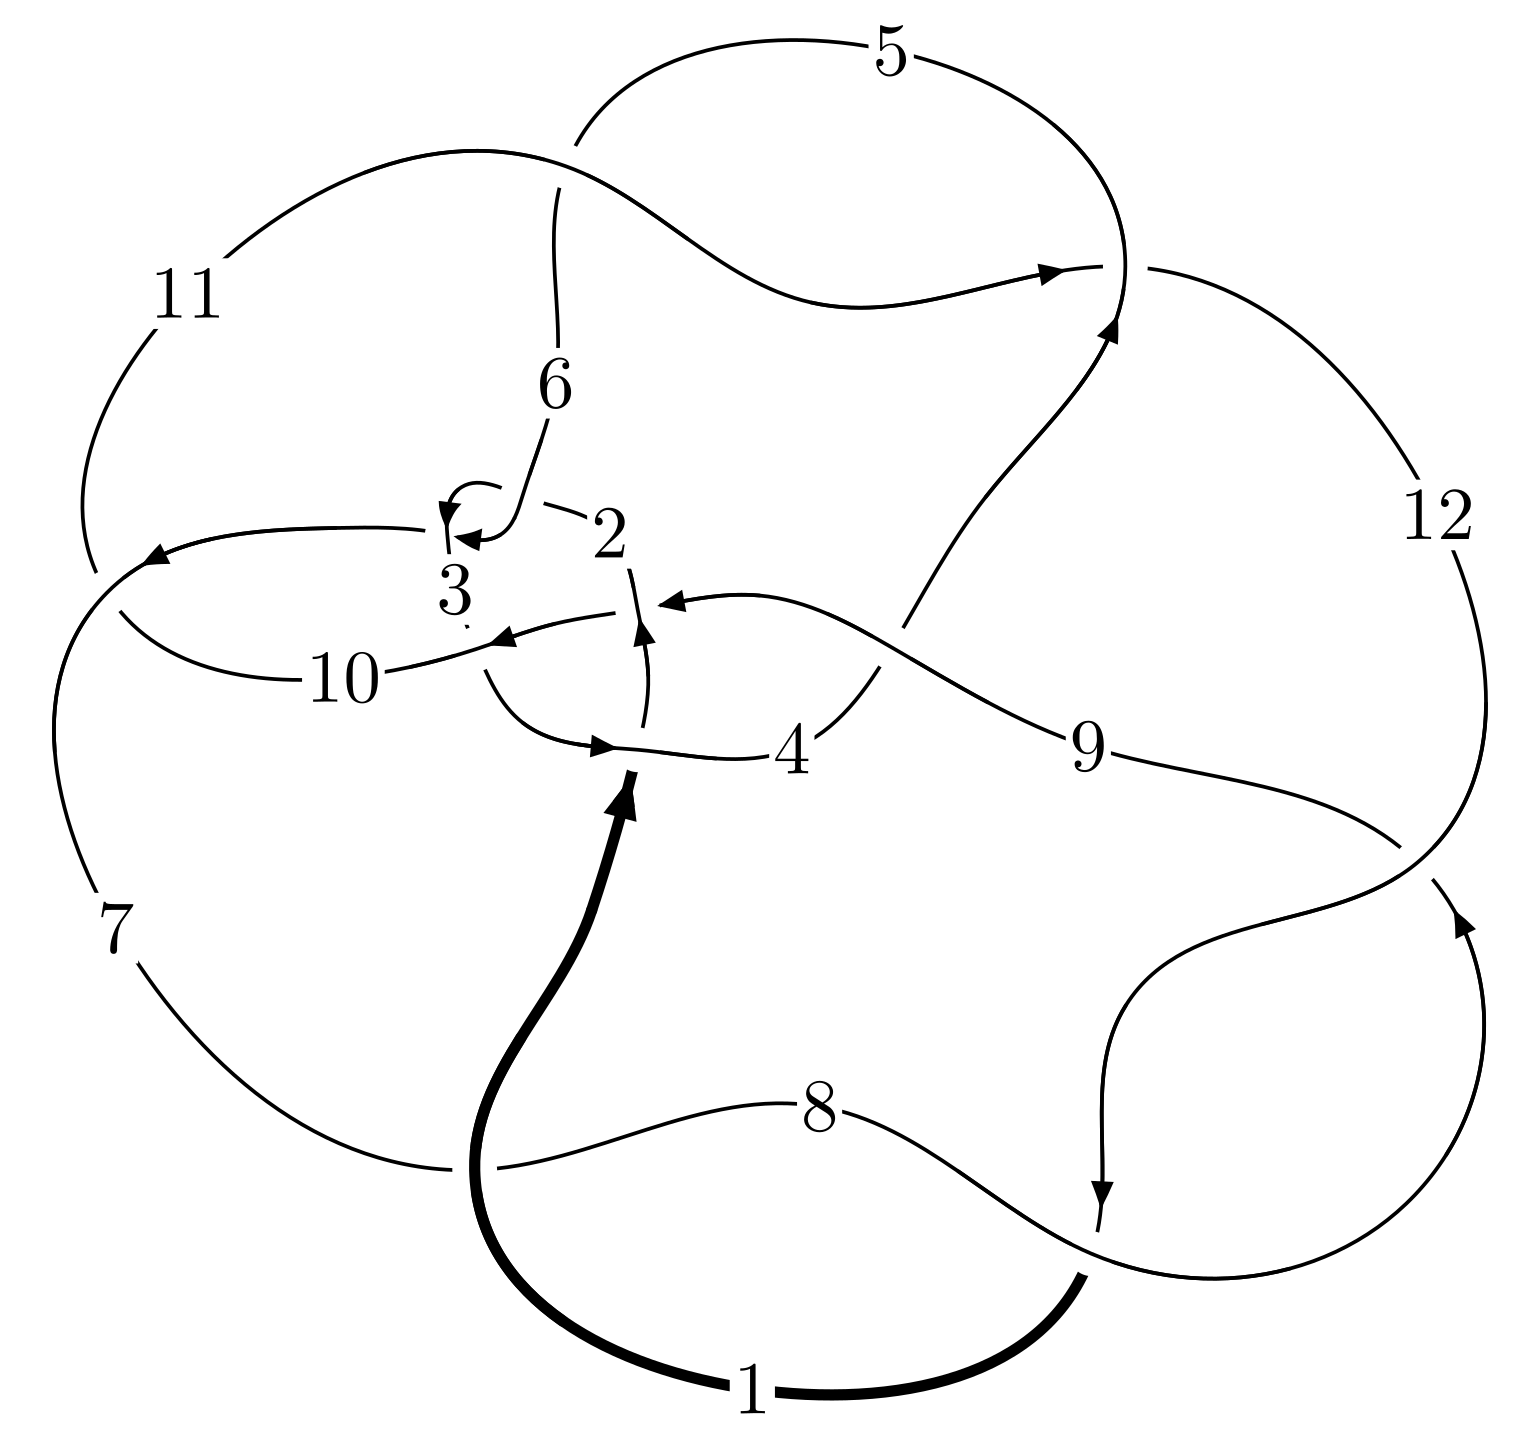
\includegraphics[width=112pt]{../../../GIT/diagram.site/Diagrams/png/1758_12a_0957.png}\\
\ \ \ A knot diagram\footnotemark}&
\allowdisplaybreaks
\textbf{Linearized knot diagam} \\
\cline{2-2}
 &
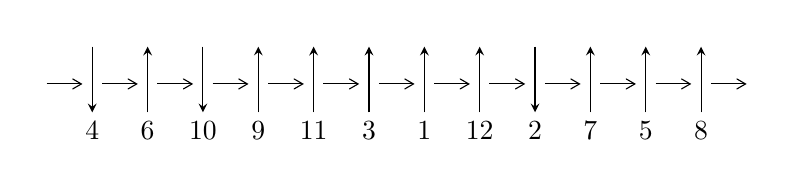
\begin{tikzpicture}[x=20pt, y=17pt]
	% nodes
	\node (C0) at (0, 0) {};
	\node (C1) at (1, 0) {};
	\node (C1U) at (1, +1) {};
	\node (C1D) at (1, -1) {4};

	\node (C2) at (2, 0) {};
	\node (C2U) at (2, +1) {};
	\node (C2D) at (2, -1) {6};

	\node (C3) at (3, 0) {};
	\node (C3U) at (3, +1) {};
	\node (C3D) at (3, -1) {10};

	\node (C4) at (4, 0) {};
	\node (C4U) at (4, +1) {};
	\node (C4D) at (4, -1) {9};

	\node (C5) at (5, 0) {};
	\node (C5U) at (5, +1) {};
	\node (C5D) at (5, -1) {11};

	\node (C6) at (6, 0) {};
	\node (C6U) at (6, +1) {};
	\node (C6D) at (6, -1) {3};

	\node (C7) at (7, 0) {};
	\node (C7U) at (7, +1) {};
	\node (C7D) at (7, -1) {1};

	\node (C8) at (8, 0) {};
	\node (C8U) at (8, +1) {};
	\node (C8D) at (8, -1) {12};

	\node (C9) at (9, 0) {};
	\node (C9U) at (9, +1) {};
	\node (C9D) at (9, -1) {2};

	\node (C10) at (10, 0) {};
	\node (C10U) at (10, +1) {};
	\node (C10D) at (10, -1) {7};

	\node (C11) at (11, 0) {};
	\node (C11U) at (11, +1) {};
	\node (C11D) at (11, -1) {5};

	\node (C12) at (12, 0) {};
	\node (C12U) at (12, +1) {};
	\node (C12D) at (12, -1) {8};
	\node (C13) at (13, 0) {};

	% arrows
	\draw[->,>={angle 60}]
	(C0) edge (C1) (C1) edge (C2) (C2) edge (C3) (C3) edge (C4) (C4) edge (C5) (C5) edge (C6) (C6) edge (C7) (C7) edge (C8) (C8) edge (C9) (C9) edge (C10) (C10) edge (C11) (C11) edge (C12) (C12) edge (C13) ;	\draw[->,>=stealth]
	(C1U) edge (C1D) (C2D) edge (C2U) (C3U) edge (C3D) (C4D) edge (C4U) (C5D) edge (C5U) (C6D) edge (C6U) (C7D) edge (C7U) (C8D) edge (C8U) (C9U) edge (C9D) (C10D) edge (C10U) (C11D) edge (C11U) (C12D) edge (C12U) ;
	\end{tikzpicture} \\
\hhline{~~} \\& 
\textbf{Solving Sequence} \\ \cline{2-2} 
 &
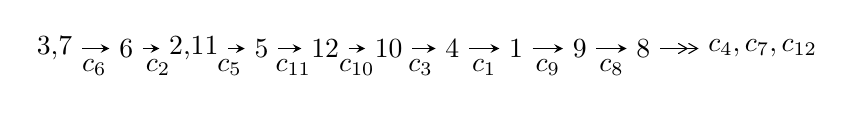
\begin{tikzpicture}[x=23pt, y=7pt]
	% node
	\node (A0) at (-1/8, 0) {3,7};
	\node (A1) at (1, 0) {6};
	\node (A2) at (33/16, 0) {2,11};
	\node (A3) at (25/8, 0) {5};
	\node (A4) at (33/8, 0) {12};
	\node (A5) at (41/8, 0) {10};
	\node (A6) at (49/8, 0) {4};
	\node (A7) at (57/8, 0) {1};
	\node (A8) at (65/8, 0) {9};
	\node (A9) at (73/8, 0) {8};
	\node (C1) at (1/2, -1) {$c_{6}$};
	\node (C2) at (3/2, -1) {$c_{2}$};
	\node (C3) at (21/8, -1) {$c_{5}$};
	\node (C4) at (29/8, -1) {$c_{11}$};
	\node (C5) at (37/8, -1) {$c_{10}$};
	\node (C6) at (45/8, -1) {$c_{3}$};
	\node (C7) at (53/8, -1) {$c_{1}$};
	\node (C8) at (61/8, -1) {$c_{9}$};
	\node (C9) at (69/8, -1) {$c_{8}$};
	\node (A10) at (11, 0) {$c_{4},c_{7},c_{12}$};

	% edge
	\draw[->,>=stealth]	
	(A0) edge (A1) (A1) edge (A2) (A2) edge (A3) (A3) edge (A4) (A4) edge (A5) (A5) edge (A6) (A6) edge (A7) (A7) edge (A8) (A8) edge (A9) ;
	\draw[->>,>={angle 60}]	
	(A9) edge (A10);
\end{tikzpicture} \\ 

\end{tabular} \\

\footnotetext{
The image of knot diagram is generated by the software ``\textbf{Draw programme}" developed by Andrew Bartholomew(\url{http://www.layer8.co.uk/maths/draw/index.htm\#Running-draw}), where we modified some parts for our purpose(\url{https://github.com/CATsTAILs/LinksPainter}).
}\phantom \\ \newline 
\centering \textbf{Ideals for irreducible components\footnotemark of $X_{\text{par}}$} 
 
\begin{align*}
I^u_{1}&=\langle 
6.01890\times10^{431} u^{131}+1.67690\times10^{432} u^{130}+\cdots+1.63556\times10^{431} b-3.45096\times10^{434},\\
\phantom{I^u_{1}}&\phantom{= \langle  }2.77517\times10^{434} u^{131}+7.86280\times10^{434} u^{130}+\cdots+3.95805\times10^{433} a-1.57625\times10^{437},\\
\phantom{I^u_{1}}&\phantom{= \langle  }u^{132}+2 u^{131}+\cdots-110 u+484\rangle \\
I^u_{2}&=\langle 
-479758582336010 u^{30}-1107917736884359 u^{29}+\cdots+2241847239778 b+2757014414903866,\\
\phantom{I^u_{2}}&\phantom{= \langle  }-371686622838711 u^{30}-869706396241666 u^{29}+\cdots+2241847239778 a+2086493761025877,\\
\phantom{I^u_{2}}&\phantom{= \langle  }u^{31}+3 u^{30}+\cdots-18 u-4\rangle \\
\\
\end{align*}
\raggedright * 2 irreducible components of $\dim_{\mathbb{C}}=0$, with total 163 representations.\\
\footnotetext{All coefficients of polynomials are rational numbers. But the coefficients are sometimes approximated in decimal forms when there is not enough margin.}
\newpage
\renewcommand{\arraystretch}{1}
\centering \section*{I. $I^u_{1}= \langle 6.02\times10^{431} u^{131}+1.68\times10^{432} u^{130}+\cdots+1.64\times10^{431} b-3.45\times10^{434},\;2.78\times10^{434} u^{131}+7.86\times10^{434} u^{130}+\cdots+3.96\times10^{433} a-1.58\times10^{437},\;u^{132}+2 u^{131}+\cdots-110 u+484 \rangle$}
\flushleft \textbf{(i) Arc colorings}\\
\begin{tabular}{m{7pt} m{180pt} m{7pt} m{180pt} }
\flushright $a_{3}=$&$\begin{pmatrix}0\\u\end{pmatrix}$ \\
\flushright $a_{7}=$&$\begin{pmatrix}1\\0\end{pmatrix}$ \\
\flushright $a_{6}=$&$\begin{pmatrix}1\\u^2\end{pmatrix}$ \\
\flushright $a_{2}=$&$\begin{pmatrix}- u\\- u^3+u\end{pmatrix}$ \\
\flushright $a_{11}=$&$\begin{pmatrix}-7.01147 u^{131}-19.8654 u^{130}+\cdots+3685.03 u+3982.40\\-3.68003 u^{131}-10.2528 u^{130}+\cdots+1843.90 u+2109.96\end{pmatrix}$ \\
\flushright $a_{5}=$&$\begin{pmatrix}-2.03352 u^{131}-6.90245 u^{130}+\cdots-18.6657 u+556.179\\-0.450600 u^{131}-1.95947 u^{130}+\cdots-634.313 u-176.903\end{pmatrix}$ \\
\flushright $a_{12}=$&$\begin{pmatrix}3.32732 u^{131}+14.7189 u^{130}+\cdots+4001.59 u+1097.20\\0.428259 u^{131}+1.23170 u^{130}+\cdots-81.7935 u-202.244\end{pmatrix}$ \\
\flushright $a_{10}=$&$\begin{pmatrix}-3.33144 u^{131}-9.61255 u^{130}+\cdots+1841.13 u+1872.44\\-3.68003 u^{131}-10.2528 u^{130}+\cdots+1843.90 u+2109.96\end{pmatrix}$ \\
\flushright $a_{4}=$&$\begin{pmatrix}-1.62545 u^{131}-4.95251 u^{130}+\cdots+818.930 u+842.032\\-0.304230 u^{131}-0.850231 u^{130}+\cdots+163.230 u+174.466\end{pmatrix}$ \\
\flushright $a_{1}=$&$\begin{pmatrix}51.7438 u^{131}+153.988 u^{130}+\cdots-20436.0 u-25629.4\\-0.942105 u^{131}-2.64416 u^{130}+\cdots+481.774 u+533.851\end{pmatrix}$ \\
\flushright $a_{9}=$&$\begin{pmatrix}-5.61696 u^{131}-15.5581 u^{130}+\cdots+3561.67 u+3459.46\\-1.96769 u^{131}-5.37684 u^{130}+\cdots+1078.36 u+1188.19\end{pmatrix}$ \\
\flushright $a_{8}=$&$\begin{pmatrix}-85.5423 u^{131}-248.486 u^{130}+\cdots+39558.0 u+45553.8\\-1.25261 u^{131}-3.59742 u^{130}+\cdots+593.297 u+683.193\end{pmatrix}$\\&\end{tabular}
\flushleft \textbf{(ii) Obstruction class $= -1$}\\~\\
\flushleft \textbf{(iii) Cusp Shapes $= 164.847 u^{131}+466.596 u^{130}+\cdots-94982.5 u-96460.8$}\\~\\
\newpage\renewcommand{\arraystretch}{1}
\flushleft \textbf{(iv) u-Polynomials at the component}\newline \\
\begin{tabular}{m{50pt}|m{274pt}}
Crossings & \hspace{64pt}u-Polynomials at each crossing \\
\hline $$\begin{aligned}c_{1}\end{aligned}$$&$\begin{aligned}
&u^{132}-5 u^{131}+\cdots+319 u-1
\end{aligned}$\\
\hline $$\begin{aligned}c_{2},c_{6}\end{aligned}$$&$\begin{aligned}
&u^{132}+2 u^{131}+\cdots-110 u+484
\end{aligned}$\\
\hline $$\begin{aligned}c_{3}\end{aligned}$$&$\begin{aligned}
&u^{132}- u^{131}+\cdots-150284 u-19367
\end{aligned}$\\
\hline $$\begin{aligned}c_{4}\end{aligned}$$&$\begin{aligned}
&u^{132}+3 u^{131}+\cdots+1603714647 u-570362249
\end{aligned}$\\
\hline $$\begin{aligned}c_{5},c_{11}\end{aligned}$$&$\begin{aligned}
&u^{132}- u^{131}+\cdots-3944517 u-299011
\end{aligned}$\\
\hline $$\begin{aligned}c_{7},c_{8},c_{12}\end{aligned}$$&$\begin{aligned}
&u^{132}+68 u^{130}+\cdots+19 u+1
\end{aligned}$\\
\hline $$\begin{aligned}c_{9}\end{aligned}$$&$\begin{aligned}
&u^{132}-2 u^{131}+\cdots+11993 u-4467
\end{aligned}$\\
\hline $$\begin{aligned}c_{10}\end{aligned}$$&$\begin{aligned}
&u^{132}+u^{131}+\cdots-5047 u+321
\end{aligned}$\\
\hline
\end{tabular}\\~\\
\newpage\renewcommand{\arraystretch}{1}
\flushleft \textbf{(v) Riley Polynomials at the component}\newline \\
\begin{tabular}{m{50pt}|m{274pt}}
Crossings & \hspace{64pt}Riley Polynomials at each crossing \\
\hline $$\begin{aligned}c_{1}\end{aligned}$$&$\begin{aligned}
&y^{132}-9 y^{131}+\cdots-100571 y+1
\end{aligned}$\\
\hline $$\begin{aligned}c_{2},c_{6}\end{aligned}$$&$\begin{aligned}
&y^{132}-72 y^{131}+\cdots-2771868 y+234256
\end{aligned}$\\
\hline $$\begin{aligned}c_{3}\end{aligned}$$&$\begin{aligned}
&y^{132}+23 y^{131}+\cdots+8515836038 y+375080689
\end{aligned}$\\
\hline $$\begin{aligned}c_{4}\end{aligned}$$&$\begin{aligned}
&y^{132}+59 y^{131}+\cdots+3.67\times10^{18} y+3.25\times10^{17}
\end{aligned}$\\
\hline $$\begin{aligned}c_{5},c_{11}\end{aligned}$$&$\begin{aligned}
&y^{132}+109 y^{131}+\cdots+89028169385 y+89407578121
\end{aligned}$\\
\hline $$\begin{aligned}c_{7},c_{8},c_{12}\end{aligned}$$&$\begin{aligned}
&y^{132}+136 y^{131}+\cdots-145 y+1
\end{aligned}$\\
\hline $$\begin{aligned}c_{9}\end{aligned}$$&$\begin{aligned}
&y^{132}+14 y^{131}+\cdots-1024697647 y+19954089
\end{aligned}$\\
\hline $$\begin{aligned}c_{10}\end{aligned}$$&$\begin{aligned}
&y^{132}+7 y^{131}+\cdots+22512797 y+103041
\end{aligned}$\\
\hline
\end{tabular}\\~\\
\newpage\flushleft \textbf{(vi) Complex Volumes and Cusp Shapes}
$$\begin{array}{c|c|c}  
\text{Solutions to }I^u_{1}& \I (\text{vol} + \sqrt{-1}CS) & \text{Cusp shape}\\
 \hline 
\begin{aligned}
u &= -0.884816 + 0.474905 I \\
a &= \phantom{-}1.66252 - 0.11441 I \\
b &= \phantom{-}0.650392 - 0.231643 I\end{aligned}
 & -3.27259 - 2.47976 I & \phantom{-0.000000 } 0 \\ \hline\begin{aligned}
u &= -0.884816 - 0.474905 I \\
a &= \phantom{-}1.66252 + 0.11441 I \\
b &= \phantom{-}0.650392 + 0.231643 I\end{aligned}
 & -3.27259 + 2.47976 I & \phantom{-0.000000 } 0 \\ \hline\begin{aligned}
u &= \phantom{-}0.915765 + 0.340582 I \\
a &= -2.80388 - 1.06421 I \\
b &= -1.58944 - 1.35988 I\end{aligned}
 & -9.50542 - 4.87494 I & \phantom{-0.000000 } 0 \\ \hline\begin{aligned}
u &= \phantom{-}0.915765 - 0.340582 I \\
a &= -2.80388 + 1.06421 I \\
b &= -1.58944 + 1.35988 I\end{aligned}
 & -9.50542 + 4.87494 I & \phantom{-0.000000 } 0 \\ \hline\begin{aligned}
u &= -0.942190 + 0.424662 I \\
a &= -2.01410 + 0.52332 I \\
b &= -0.487234 + 0.684826 I\end{aligned}
 & -3.41617 - 6.49521 I & \phantom{-0.000000 } 0 \\ \hline\begin{aligned}
u &= -0.942190 - 0.424662 I \\
a &= -2.01410 - 0.52332 I \\
b &= -0.487234 - 0.684826 I\end{aligned}
 & -3.41617 + 6.49521 I & \phantom{-0.000000 } 0 \\ \hline\begin{aligned}
u &= -0.386658 + 0.884802 I \\
a &= -0.045284 + 0.449711 I \\
b &= \phantom{-}0.756898 + 0.730603 I\end{aligned}
 & -3.48885 + 1.37931 I & \phantom{-0.000000 } 0 \\ \hline\begin{aligned}
u &= -0.386658 - 0.884802 I \\
a &= -0.045284 - 0.449711 I \\
b &= \phantom{-}0.756898 - 0.730603 I\end{aligned}
 & -3.48885 - 1.37931 I & \phantom{-0.000000 } 0 \\ \hline\begin{aligned}
u &= -0.967695 + 0.409732 I \\
a &= \phantom{-}2.12999 - 0.80994 I \\
b &= \phantom{-}0.296010 - 0.830334 I\end{aligned}
 & -9.89787 - 9.67184 I & \phantom{-0.000000 } 0 \\ \hline\begin{aligned}
u &= -0.967695 - 0.409732 I \\
a &= \phantom{-}2.12999 + 0.80994 I \\
b &= \phantom{-}0.296010 + 0.830334 I\end{aligned}
 & -9.89787 + 9.67184 I & \phantom{-0.000000 } 0\\
 \hline 
 \end{array}$$\newpage$$\begin{array}{c|c|c}  
\text{Solutions to }I^u_{1}& \I (\text{vol} + \sqrt{-1}CS) & \text{Cusp shape}\\
 \hline 
\begin{aligned}
u &= -0.789295 + 0.515215 I \\
a &= -1.19236 - 1.38844 I \\
b &= -1.32264 - 1.05992 I\end{aligned}
 & -8.63511 - 2.84252 I & \phantom{-0.000000 } 0 \\ \hline\begin{aligned}
u &= -0.789295 - 0.515215 I \\
a &= -1.19236 + 1.38844 I \\
b &= -1.32264 + 1.05992 I\end{aligned}
 & -8.63511 + 2.84252 I & \phantom{-0.000000 } 0 \\ \hline\begin{aligned}
u &= \phantom{-}0.938691 + 0.059442 I \\
a &= \phantom{-}4.15791 + 3.69908 I \\
b &= \phantom{-}0.191248 - 0.131579 I\end{aligned}
 & -5.07473 + 0.16829 I & \phantom{-0.000000 } 0 \\ \hline\begin{aligned}
u &= \phantom{-}0.938691 - 0.059442 I \\
a &= \phantom{-}4.15791 - 3.69908 I \\
b &= \phantom{-}0.191248 + 0.131579 I\end{aligned}
 & -5.07473 - 0.16829 I & \phantom{-0.000000 } 0 \\ \hline\begin{aligned}
u &= \phantom{-}0.989571 + 0.388105 I \\
a &= \phantom{-}1.45147 - 0.41211 I \\
b &= \phantom{-}1.06468 + 1.35709 I\end{aligned}
 & -1.11664 + 5.62858 I & \phantom{-0.000000 } 0 \\ \hline\begin{aligned}
u &= \phantom{-}0.989571 - 0.388105 I \\
a &= \phantom{-}1.45147 + 0.41211 I \\
b &= \phantom{-}1.06468 - 1.35709 I\end{aligned}
 & -1.11664 - 5.62858 I & \phantom{-0.000000 } 0 \\ \hline\begin{aligned}
u &= -0.775797 + 0.512353 I \\
a &= \phantom{-}1.35566 + 0.77126 I \\
b &= \phantom{-}1.056800 + 0.533841 I\end{aligned}
 & -3.35318 - 2.09628 I & \phantom{-0.000000 } 0 \\ \hline\begin{aligned}
u &= -0.775797 - 0.512353 I \\
a &= \phantom{-}1.35566 - 0.77126 I \\
b &= \phantom{-}1.056800 - 0.533841 I\end{aligned}
 & -3.35318 + 2.09628 I & \phantom{-0.000000 } 0 \\ \hline\begin{aligned}
u &= \phantom{-}0.246759 + 0.895153 I \\
a &= \phantom{-}0.086715 + 0.519405 I \\
b &= -0.290111 - 0.018909 I\end{aligned}
 & -1.15474 + 1.23049 I & \phantom{-0.000000 } 0 \\ \hline\begin{aligned}
u &= \phantom{-}0.246759 - 0.895153 I \\
a &= \phantom{-}0.086715 - 0.519405 I \\
b &= -0.290111 + 0.018909 I\end{aligned}
 & -1.15474 - 1.23049 I & \phantom{-0.000000 } 0\\
 \hline 
 \end{array}$$\newpage$$\begin{array}{c|c|c}  
\text{Solutions to }I^u_{1}& \I (\text{vol} + \sqrt{-1}CS) & \text{Cusp shape}\\
 \hline 
\begin{aligned}
u &= \phantom{-}0.908416 + 0.190893 I \\
a &= -1.70213 - 0.54652 I \\
b &= -0.970588 + 0.555808 I\end{aligned}
 & -0.983366 + 0.894266 I & \phantom{-0.000000 } 0 \\ \hline\begin{aligned}
u &= \phantom{-}0.908416 - 0.190893 I \\
a &= -1.70213 + 0.54652 I \\
b &= -0.970588 - 0.555808 I\end{aligned}
 & -0.983366 - 0.894266 I & \phantom{-0.000000 } 0 \\ \hline\begin{aligned}
u &= \phantom{-}0.008635 + 0.928101 I \\
a &= -0.144296 + 0.342857 I \\
b &= -1.009900 - 0.536885 I\end{aligned}
 & -5.60921 + 7.00889 I & \phantom{-0.000000 } 0 \\ \hline\begin{aligned}
u &= \phantom{-}0.008635 - 0.928101 I \\
a &= -0.144296 - 0.342857 I \\
b &= -1.009900 + 0.536885 I\end{aligned}
 & -5.60921 - 7.00889 I & \phantom{-0.000000 } 0 \\ \hline\begin{aligned}
u &= \phantom{-}0.883314 + 0.281049 I \\
a &= \phantom{-}2.58613 + 0.89656 I \\
b &= \phantom{-}1.31484 + 0.80921 I\end{aligned}
 & -2.53291 - 2.22174 I & \phantom{-0.000000 } 0 \\ \hline\begin{aligned}
u &= \phantom{-}0.883314 - 0.281049 I \\
a &= \phantom{-}2.58613 - 0.89656 I \\
b &= \phantom{-}1.31484 - 0.80921 I\end{aligned}
 & -2.53291 + 2.22174 I & \phantom{-0.000000 } 0 \\ \hline\begin{aligned}
u &= -1.055710 + 0.263342 I \\
a &= \phantom{-}2.01783 + 0.09373 I \\
b &= \phantom{-}1.53656 - 0.78293 I\end{aligned}
 & -0.85765 - 5.45781 I & \phantom{-0.000000 } 0 \\ \hline\begin{aligned}
u &= -1.055710 - 0.263342 I \\
a &= \phantom{-}2.01783 - 0.09373 I \\
b &= \phantom{-}1.53656 + 0.78293 I\end{aligned}
 & -0.85765 + 5.45781 I & \phantom{-0.000000 } 0 \\ \hline\begin{aligned}
u &= \phantom{-}0.866590 + 0.210032 I \\
a &= \phantom{-}0.71853 - 1.34233 I \\
b &= \phantom{-}0.93448 - 2.06252 I\end{aligned}
 & -2.74406 + 4.51032 I & \phantom{-0.000000 } 0 \\ \hline\begin{aligned}
u &= \phantom{-}0.866590 - 0.210032 I \\
a &= \phantom{-}0.71853 + 1.34233 I \\
b &= \phantom{-}0.93448 + 2.06252 I\end{aligned}
 & -2.74406 - 4.51032 I & \phantom{-0.000000 } 0\\
 \hline 
 \end{array}$$\newpage$$\begin{array}{c|c|c}  
\text{Solutions to }I^u_{1}& \I (\text{vol} + \sqrt{-1}CS) & \text{Cusp shape}\\
 \hline 
\begin{aligned}
u &= \phantom{-}0.013820 + 0.888222 I \\
a &= -0.049782 - 0.384372 I \\
b &= \phantom{-}0.773005 + 0.387860 I\end{aligned}
 & \phantom{-}0.32452 + 4.34292 I & \phantom{-0.000000 } 0 \\ \hline\begin{aligned}
u &= \phantom{-}0.013820 - 0.888222 I \\
a &= -0.049782 + 0.384372 I \\
b &= \phantom{-}0.773005 - 0.387860 I\end{aligned}
 & \phantom{-}0.32452 - 4.34292 I & \phantom{-0.000000 } 0 \\ \hline\begin{aligned}
u &= \phantom{-}1.095560 + 0.190155 I \\
a &= -1.54685 + 0.71390 I \\
b &= -0.224526 - 0.518265 I\end{aligned}
 & -3.99476 + 0.29972 I & \phantom{-0.000000 } 0 \\ \hline\begin{aligned}
u &= \phantom{-}1.095560 - 0.190155 I \\
a &= -1.54685 - 0.71390 I \\
b &= -0.224526 + 0.518265 I\end{aligned}
 & -3.99476 - 0.29972 I & \phantom{-0.000000 } 0 \\ \hline\begin{aligned}
u &= \phantom{-}1.059130 + 0.375973 I \\
a &= -1.166780 + 0.693723 I \\
b &= -0.997325 - 0.841214 I\end{aligned}
 & \phantom{-}3.18035 + 2.90322 I & \phantom{-0.000000 } 0 \\ \hline\begin{aligned}
u &= \phantom{-}1.059130 - 0.375973 I \\
a &= -1.166780 - 0.693723 I \\
b &= -0.997325 + 0.841214 I\end{aligned}
 & \phantom{-}3.18035 - 2.90322 I & \phantom{-0.000000 } 0 \\ \hline\begin{aligned}
u &= -0.724711 + 0.487676 I \\
a &= -2.08125 - 0.81701 I \\
b &= -1.57151 - 0.05639 I\end{aligned}
 & -8.81589 - 1.30826 I & \phantom{-0.000000 } 0 \\ \hline\begin{aligned}
u &= -0.724711 - 0.487676 I \\
a &= -2.08125 + 0.81701 I \\
b &= -1.57151 + 0.05639 I\end{aligned}
 & -8.81589 + 1.30826 I & \phantom{-0.000000 } 0 \\ \hline\begin{aligned}
u &= -1.132960 + 0.135239 I \\
a &= -1.49657 + 0.19781 I \\
b &= -1.29493 + 0.87121 I\end{aligned}
 & \phantom{-}4.49382 - 1.59161 I & \phantom{-0.000000 } 0 \\ \hline\begin{aligned}
u &= -1.132960 - 0.135239 I \\
a &= -1.49657 - 0.19781 I \\
b &= -1.29493 - 0.87121 I\end{aligned}
 & \phantom{-}4.49382 + 1.59161 I & \phantom{-0.000000 } 0\\
 \hline 
 \end{array}$$\newpage$$\begin{array}{c|c|c}  
\text{Solutions to }I^u_{1}& \I (\text{vol} + \sqrt{-1}CS) & \text{Cusp shape}\\
 \hline 
\begin{aligned}
u &= \phantom{-}0.851977\phantom{ +0.000000I} \\
a &= -3.75966\phantom{ +0.000000I} \\
b &= -0.269385\phantom{ +0.000000I}\end{aligned}
 & -0.410229\phantom{ +0.000000I} & \phantom{-0.000000 } 0 \\ \hline\begin{aligned}
u &= \phantom{-}1.097330 + 0.351337 I \\
a &= -0.284882 - 0.826418 I \\
b &= \phantom{-}0.564404 - 0.176494 I\end{aligned}
 & -2.48106 - 0.05788 I & \phantom{-0.000000 } 0 \\ \hline\begin{aligned}
u &= \phantom{-}1.097330 - 0.351337 I \\
a &= -0.284882 + 0.826418 I \\
b &= \phantom{-}0.564404 + 0.176494 I\end{aligned}
 & -2.48106 + 0.05788 I & \phantom{-0.000000 } 0 \\ \hline\begin{aligned}
u &= \phantom{-}0.247341 + 1.128890 I \\
a &= \phantom{-}0.116446 + 0.457801 I \\
b &= -0.866422 + 0.994465 I\end{aligned}
 & -11.1165 - 12.7107 I & \phantom{-0.000000 } 0 \\ \hline\begin{aligned}
u &= \phantom{-}0.247341 - 1.128890 I \\
a &= \phantom{-}0.116446 - 0.457801 I \\
b &= -0.866422 - 0.994465 I\end{aligned}
 & -11.1165 + 12.7107 I & \phantom{-0.000000 } 0 \\ \hline\begin{aligned}
u &= -0.803523 + 0.833951 I \\
a &= \phantom{-}0.440111 + 0.803172 I \\
b &= \phantom{-}1.193060 + 0.417998 I\end{aligned}
 & -3.01450 + 1.23639 I & \phantom{-0.000000 } 0 \\ \hline\begin{aligned}
u &= -0.803523 - 0.833951 I \\
a &= \phantom{-}0.440111 - 0.803172 I \\
b &= \phantom{-}1.193060 - 0.417998 I\end{aligned}
 & -3.01450 - 1.23639 I & \phantom{-0.000000 } 0 \\ \hline\begin{aligned}
u &= \phantom{-}1.127780 + 0.271409 I \\
a &= \phantom{-}1.028370 - 0.542660 I \\
b &= \phantom{-}0.496725 + 0.498862 I\end{aligned}
 & \phantom{-}1.75805 + 1.07231 I & \phantom{-0.000000 } 0 \\ \hline\begin{aligned}
u &= \phantom{-}1.127780 - 0.271409 I \\
a &= \phantom{-}1.028370 + 0.542660 I \\
b &= \phantom{-}0.496725 - 0.498862 I\end{aligned}
 & \phantom{-}1.75805 - 1.07231 I & \phantom{-0.000000 } 0 \\ \hline\begin{aligned}
u &= -1.103060 + 0.367632 I \\
a &= \phantom{-}0.573973 - 0.933648 I \\
b &= \phantom{-}0.17795 - 1.57989 I\end{aligned}
 & -5.07414 - 5.28950 I & \phantom{-0.000000 } 0\\
 \hline 
 \end{array}$$\newpage$$\begin{array}{c|c|c}  
\text{Solutions to }I^u_{1}& \I (\text{vol} + \sqrt{-1}CS) & \text{Cusp shape}\\
 \hline 
\begin{aligned}
u &= -1.103060 - 0.367632 I \\
a &= \phantom{-}0.573973 + 0.933648 I \\
b &= \phantom{-}0.17795 + 1.57989 I\end{aligned}
 & -5.07414 + 5.28950 I & \phantom{-0.000000 } 0 \\ \hline\begin{aligned}
u &= -1.015100 + 0.573103 I \\
a &= -0.964303 + 0.590903 I \\
b &= -0.0171108 + 0.0735246 I\end{aligned}
 & -8.63379 + 1.07483 I & \phantom{-0.000000 } 0 \\ \hline\begin{aligned}
u &= -1.015100 - 0.573103 I \\
a &= -0.964303 - 0.590903 I \\
b &= -0.0171108 - 0.0735246 I\end{aligned}
 & -8.63379 - 1.07483 I & \phantom{-0.000000 } 0 \\ \hline\begin{aligned}
u &= \phantom{-}0.787789 + 0.210688 I \\
a &= -0.05832 + 2.35922 I \\
b &= -0.61444 + 2.74989 I\end{aligned}
 & -10.14810 + 7.50183 I & \phantom{-0.000000 } 0 \\ \hline\begin{aligned}
u &= \phantom{-}0.787789 - 0.210688 I \\
a &= -0.05832 - 2.35922 I \\
b &= -0.61444 - 2.74989 I\end{aligned}
 & -10.14810 - 7.50183 I & \phantom{-0.000000 } 0 \\ \hline\begin{aligned}
u &= \phantom{-}1.128850 + 0.404643 I \\
a &= \phantom{-}0.93270 - 1.09980 I \\
b &= \phantom{-}1.194680 + 0.318888 I\end{aligned}
 & -0.445813 + 1.114960 I & \phantom{-0.000000 } 0 \\ \hline\begin{aligned}
u &= \phantom{-}1.128850 - 0.404643 I \\
a &= \phantom{-}0.93270 + 1.09980 I \\
b &= \phantom{-}1.194680 - 0.318888 I\end{aligned}
 & -0.445813 - 1.114960 I & \phantom{-0.000000 } 0 \\ \hline\begin{aligned}
u &= \phantom{-}0.282513 + 1.169350 I \\
a &= -0.116569 - 0.443418 I \\
b &= \phantom{-}0.770994 - 0.837968 I\end{aligned}
 & -4.14351 - 8.21803 I & \phantom{-0.000000 } 0 \\ \hline\begin{aligned}
u &= \phantom{-}0.282513 - 1.169350 I \\
a &= -0.116569 + 0.443418 I \\
b &= \phantom{-}0.770994 + 0.837968 I\end{aligned}
 & -4.14351 + 8.21803 I & \phantom{-0.000000 } 0 \\ \hline\begin{aligned}
u &= \phantom{-}1.138750 + 0.399109 I \\
a &= -0.378575 + 0.658815 I \\
b &= -0.722084 - 0.146977 I\end{aligned}
 & \phantom{-}2.77717 + 1.00054 I & \phantom{-0.000000 } 0\\
 \hline 
 \end{array}$$\newpage$$\begin{array}{c|c|c}  
\text{Solutions to }I^u_{1}& \I (\text{vol} + \sqrt{-1}CS) & \text{Cusp shape}\\
 \hline 
\begin{aligned}
u &= \phantom{-}1.138750 - 0.399109 I \\
a &= -0.378575 - 0.658815 I \\
b &= -0.722084 + 0.146977 I\end{aligned}
 & \phantom{-}2.77717 - 1.00054 I & \phantom{-0.000000 } 0 \\ \hline\begin{aligned}
u &= -0.526152 + 0.576468 I \\
a &= \phantom{-}0.558429 + 0.122035 I \\
b &= \phantom{-}0.045335 + 1.035590 I\end{aligned}
 & -4.20850 - 1.73518 I & \phantom{-0.000000 } 0 \\ \hline\begin{aligned}
u &= -0.526152 - 0.576468 I \\
a &= \phantom{-}0.558429 - 0.122035 I \\
b &= \phantom{-}0.045335 - 1.035590 I\end{aligned}
 & -4.20850 + 1.73518 I & \phantom{-0.000000 } 0 \\ \hline\begin{aligned}
u &= -1.126290 + 0.537145 I \\
a &= \phantom{-}1.84916 + 0.33181 I \\
b &= \phantom{-}1.61023 - 0.93755 I\end{aligned}
 & -1.29258 - 6.51091 I & \phantom{-0.000000 } 0 \\ \hline\begin{aligned}
u &= -1.126290 - 0.537145 I \\
a &= \phantom{-}1.84916 - 0.33181 I \\
b &= \phantom{-}1.61023 + 0.93755 I\end{aligned}
 & -1.29258 + 6.51091 I & \phantom{-0.000000 } 0 \\ \hline\begin{aligned}
u &= -0.164749 + 0.733190 I \\
a &= \phantom{-}0.643439 - 0.216613 I \\
b &= -0.601698 - 1.000480 I\end{aligned}
 & -0.90911 + 2.58269 I & \phantom{-0.000000 } 0 \\ \hline\begin{aligned}
u &= -0.164749 - 0.733190 I \\
a &= \phantom{-}0.643439 + 0.216613 I \\
b &= -0.601698 + 1.000480 I\end{aligned}
 & -0.90911 - 2.58269 I & \phantom{-0.000000 } 0 \\ \hline\begin{aligned}
u &= \phantom{-}1.208830 + 0.326446 I \\
a &= \phantom{-}2.08876 + 0.89815 I \\
b &= \phantom{-}1.85882 + 1.43889 I\end{aligned}
 & -6.31828 + 8.77435 I & \phantom{-0.000000 } 0 \\ \hline\begin{aligned}
u &= \phantom{-}1.208830 - 0.326446 I \\
a &= \phantom{-}2.08876 - 0.89815 I \\
b &= \phantom{-}1.85882 - 1.43889 I\end{aligned}
 & -6.31828 - 8.77435 I & \phantom{-0.000000 } 0 \\ \hline\begin{aligned}
u &= -0.179678 + 0.722554 I \\
a &= -0.929904 + 0.391490 I \\
b &= \phantom{-}0.60150 + 1.35100 I\end{aligned}
 & -6.22703 + 3.42085 I & \phantom{-0.000000 } 0\\
 \hline 
 \end{array}$$\newpage$$\begin{array}{c|c|c}  
\text{Solutions to }I^u_{1}& \I (\text{vol} + \sqrt{-1}CS) & \text{Cusp shape}\\
 \hline 
\begin{aligned}
u &= -0.179678 - 0.722554 I \\
a &= -0.929904 - 0.391490 I \\
b &= \phantom{-}0.60150 - 1.35100 I\end{aligned}
 & -6.22703 - 3.42085 I & \phantom{-0.000000 } 0 \\ \hline\begin{aligned}
u &= -1.157780 + 0.499932 I \\
a &= \phantom{-}2.05361 - 0.46284 I \\
b &= \phantom{-}1.50176 - 1.67005 I\end{aligned}
 & -3.39124 - 8.01755 I & \phantom{-0.000000 } 0 \\ \hline\begin{aligned}
u &= -1.157780 - 0.499932 I \\
a &= \phantom{-}2.05361 + 0.46284 I \\
b &= \phantom{-}1.50176 + 1.67005 I\end{aligned}
 & -3.39124 + 8.01755 I & \phantom{-0.000000 } 0 \\ \hline\begin{aligned}
u &= -1.020200 + 0.752092 I \\
a &= -1.030420 - 0.695273 I \\
b &= -1.400400 + 0.146934 I\end{aligned}
 & \phantom{-}1.07326 - 3.01270 I & \phantom{-0.000000 } 0 \\ \hline\begin{aligned}
u &= -1.020200 - 0.752092 I \\
a &= -1.030420 + 0.695273 I \\
b &= -1.400400 - 0.146934 I\end{aligned}
 & \phantom{-}1.07326 + 3.01270 I & \phantom{-0.000000 } 0 \\ \hline\begin{aligned}
u &= -1.166740 + 0.501144 I \\
a &= -1.84066 + 0.18303 I \\
b &= -1.40640 + 1.36274 I\end{aligned}
 & \phantom{-}2.00072 - 7.20882 I & \phantom{-0.000000 } 0 \\ \hline\begin{aligned}
u &= -1.166740 - 0.501144 I \\
a &= -1.84066 - 0.18303 I \\
b &= -1.40640 - 1.36274 I\end{aligned}
 & \phantom{-}2.00072 + 7.20882 I & \phantom{-0.000000 } 0 \\ \hline\begin{aligned}
u &= -1.268970 + 0.048065 I \\
a &= \phantom{-}0.499876 + 0.218152 I \\
b &= \phantom{-}0.522206 + 0.829263 I\end{aligned}
 & \phantom{-}3.21693 - 3.39726 I & \phantom{-0.000000 } 0 \\ \hline\begin{aligned}
u &= -1.268970 - 0.048065 I \\
a &= \phantom{-}0.499876 - 0.218152 I \\
b &= \phantom{-}0.522206 - 0.829263 I\end{aligned}
 & \phantom{-}3.21693 + 3.39726 I & \phantom{-0.000000 } 0 \\ \hline\begin{aligned}
u &= \phantom{-}0.274668 + 1.257710 I \\
a &= \phantom{-}0.116896 + 0.411868 I \\
b &= -0.561626 + 0.711698 I\end{aligned}
 & -4.51046 - 2.07669 I & \phantom{-0.000000 } 0\\
 \hline 
 \end{array}$$\newpage$$\begin{array}{c|c|c}  
\text{Solutions to }I^u_{1}& \I (\text{vol} + \sqrt{-1}CS) & \text{Cusp shape}\\
 \hline 
\begin{aligned}
u &= \phantom{-}0.274668 - 1.257710 I \\
a &= \phantom{-}0.116896 - 0.411868 I \\
b &= -0.561626 - 0.711698 I\end{aligned}
 & -4.51046 + 2.07669 I & \phantom{-0.000000 } 0 \\ \hline\begin{aligned}
u &= \phantom{-}0.589575 + 0.386588 I \\
a &= -1.57748 - 0.89380 I \\
b &= \phantom{-}0.455789 - 0.714399 I\end{aligned}
 & -2.32018 - 2.26770 I & \phantom{-0.000000 } 0 \\ \hline\begin{aligned}
u &= \phantom{-}0.589575 - 0.386588 I \\
a &= -1.57748 + 0.89380 I \\
b &= \phantom{-}0.455789 + 0.714399 I\end{aligned}
 & -2.32018 + 2.26770 I & \phantom{-0.000000 } 0 \\ \hline\begin{aligned}
u &= -0.550035 + 0.436106 I \\
a &= -0.103224 + 0.164424 I \\
b &= -0.188068 - 1.347500 I\end{aligned}
 & -4.53992 + 2.81085 I & \phantom{-0.000000 } 0 \\ \hline\begin{aligned}
u &= -0.550035 - 0.436106 I \\
a &= -0.103224 - 0.164424 I \\
b &= -0.188068 + 1.347500 I\end{aligned}
 & -4.53992 - 2.81085 I & \phantom{-0.000000 } 0 \\ \hline\begin{aligned}
u &= -0.323208 + 0.619235 I \\
a &= -0.887634 - 0.224841 I \\
b &= \phantom{-}0.342063 - 1.105550 I\end{aligned}
 & -10.47340 - 5.69331 I & \phantom{-0.000000 } 0 \\ \hline\begin{aligned}
u &= -0.323208 - 0.619235 I \\
a &= -0.887634 + 0.224841 I \\
b &= \phantom{-}0.342063 + 1.105550 I\end{aligned}
 & -10.47340 + 5.69331 I & \phantom{-0.000000 } 0 \\ \hline\begin{aligned}
u &= -1.238340 + 0.440198 I \\
a &= -0.898733 - 0.063698 I \\
b &= -0.711498 + 0.948497 I\end{aligned}
 & \phantom{-}2.94539 - 5.54607 I & \phantom{-0.000000 } 0 \\ \hline\begin{aligned}
u &= -1.238340 - 0.440198 I \\
a &= -0.898733 + 0.063698 I \\
b &= -0.711498 - 0.948497 I\end{aligned}
 & \phantom{-}2.94539 + 5.54607 I & \phantom{-0.000000 } 0 \\ \hline\begin{aligned}
u &= \phantom{-}0.144776 + 1.326740 I \\
a &= -0.162276 - 0.360508 I \\
b &= \phantom{-}0.150959 - 0.753969 I\end{aligned}
 & -12.87830 + 2.12922 I & \phantom{-0.000000 } 0\\
 \hline 
 \end{array}$$\newpage$$\begin{array}{c|c|c}  
\text{Solutions to }I^u_{1}& \I (\text{vol} + \sqrt{-1}CS) & \text{Cusp shape}\\
 \hline 
\begin{aligned}
u &= \phantom{-}0.144776 - 1.326740 I \\
a &= -0.162276 + 0.360508 I \\
b &= \phantom{-}0.150959 + 0.753969 I\end{aligned}
 & -12.87830 - 2.12922 I & \phantom{-0.000000 } 0 \\ \hline\begin{aligned}
u &= -1.250160 + 0.474407 I \\
a &= \phantom{-}1.263590 + 0.359909 I \\
b &= \phantom{-}1.010330 - 0.836469 I\end{aligned}
 & \phantom{-}4.11592 - 9.15779 I & \phantom{-0.000000 } 0 \\ \hline\begin{aligned}
u &= -1.250160 - 0.474407 I \\
a &= \phantom{-}1.263590 - 0.359909 I \\
b &= \phantom{-}1.010330 + 0.836469 I\end{aligned}
 & \phantom{-}4.11592 + 9.15779 I & \phantom{-0.000000 } 0 \\ \hline\begin{aligned}
u &= -0.546041 + 0.360490 I \\
a &= -0.095680 - 0.643072 I \\
b &= \phantom{-}0.13621 + 1.50477 I\end{aligned}
 & -11.16580 + 6.20485 I & \phantom{-0.000000 } 0 \\ \hline\begin{aligned}
u &= -0.546041 - 0.360490 I \\
a &= -0.095680 + 0.643072 I \\
b &= \phantom{-}0.13621 - 1.50477 I\end{aligned}
 & -11.16580 - 6.20485 I & \phantom{-0.000000 } 0 \\ \hline\begin{aligned}
u &= -1.266490 + 0.484120 I \\
a &= -1.50902 - 0.46555 I \\
b &= -1.15695 + 0.81499 I\end{aligned}
 & -1.73795 - 11.98760 I & \phantom{-0.000000 } 0 \\ \hline\begin{aligned}
u &= -1.266490 - 0.484120 I \\
a &= -1.50902 + 0.46555 I \\
b &= -1.15695 - 0.81499 I\end{aligned}
 & -1.73795 + 11.98760 I & \phantom{-0.000000 } 0 \\ \hline\begin{aligned}
u &= -1.190310 + 0.667724 I \\
a &= \phantom{-}1.360860 + 0.257878 I \\
b &= \phantom{-}1.235540 - 0.643906 I\end{aligned}
 & -1.32829 - 7.15022 I & \phantom{-0.000000 } 0 \\ \hline\begin{aligned}
u &= -1.190310 - 0.667724 I \\
a &= \phantom{-}1.360860 - 0.257878 I \\
b &= \phantom{-}1.235540 + 0.643906 I\end{aligned}
 & -1.32829 + 7.15022 I & \phantom{-0.000000 } 0 \\ \hline\begin{aligned}
u &= \phantom{-}1.296540 + 0.446713 I \\
a &= \phantom{-}0.974729 - 0.284396 I \\
b &= \phantom{-}0.987903 + 0.232577 I\end{aligned}
 & \phantom{-}4.26868 + 0.61252 I & \phantom{-0.000000 } 0\\
 \hline 
 \end{array}$$\newpage$$\begin{array}{c|c|c}  
\text{Solutions to }I^u_{1}& \I (\text{vol} + \sqrt{-1}CS) & \text{Cusp shape}\\
 \hline 
\begin{aligned}
u &= \phantom{-}1.296540 - 0.446713 I \\
a &= \phantom{-}0.974729 + 0.284396 I \\
b &= \phantom{-}0.987903 - 0.232577 I\end{aligned}
 & \phantom{-}4.26868 - 0.61252 I & \phantom{-0.000000 } 0 \\ \hline\begin{aligned}
u &= \phantom{-}1.364210 + 0.170896 I \\
a &= -0.87983 - 1.51138 I \\
b &= -0.81179 - 1.93774 I\end{aligned}
 & \phantom{-}1.50304 + 3.78464 I & \phantom{-0.000000 } 0 \\ \hline\begin{aligned}
u &= \phantom{-}1.364210 - 0.170896 I \\
a &= -0.87983 + 1.51138 I \\
b &= -0.81179 + 1.93774 I\end{aligned}
 & \phantom{-}1.50304 - 3.78464 I & \phantom{-0.000000 } 0 \\ \hline\begin{aligned}
u &= \phantom{-}0.615040\phantom{ +0.000000I} \\
a &= \phantom{-}1.23931\phantom{ +0.000000I} \\
b &= -0.150084\phantom{ +0.000000I}\end{aligned}
 & \phantom{-}0.986986\phantom{ +0.000000I} & \phantom{-}12.0140\phantom{ +0.000000I} \\ \hline\begin{aligned}
u &= \phantom{-}1.313880 + 0.471463 I \\
a &= -1.001950 - 0.183902 I \\
b &= -0.964616 - 0.717334 I\end{aligned}
 & \phantom{-}2.54855 + 4.26966 I & \phantom{-0.000000 } 0 \\ \hline\begin{aligned}
u &= \phantom{-}1.313880 - 0.471463 I \\
a &= -1.001950 + 0.183902 I \\
b &= -0.964616 + 0.717334 I\end{aligned}
 & \phantom{-}2.54855 - 4.26966 I & \phantom{-0.000000 } 0 \\ \hline\begin{aligned}
u &= \phantom{-}1.34776 + 0.47205 I \\
a &= -0.872535 + 0.571039 I \\
b &= -0.959679 + 0.155122 I\end{aligned}
 & -1.55609 - 1.83793 I & \phantom{-0.000000 } 0 \\ \hline\begin{aligned}
u &= \phantom{-}1.34776 - 0.47205 I \\
a &= -0.872535 - 0.571039 I \\
b &= -0.959679 - 0.155122 I\end{aligned}
 & -1.55609 + 1.83793 I & \phantom{-0.000000 } 0 \\ \hline\begin{aligned}
u &= \phantom{-}1.28250 + 0.63254 I \\
a &= -1.66972 - 0.06091 I \\
b &= -1.43305 - 1.21167 I\end{aligned}
 & -7.8525 + 18.9295 I & \phantom{-0.000000 } 0 \\ \hline\begin{aligned}
u &= \phantom{-}1.28250 - 0.63254 I \\
a &= -1.66972 + 0.06091 I \\
b &= -1.43305 + 1.21167 I\end{aligned}
 & -7.8525 - 18.9295 I & \phantom{-0.000000 } 0\\
 \hline 
 \end{array}$$\newpage$$\begin{array}{c|c|c}  
\text{Solutions to }I^u_{1}& \I (\text{vol} + \sqrt{-1}CS) & \text{Cusp shape}\\
 \hline 
\begin{aligned}
u &= -0.230142 + 0.514693 I \\
a &= -1.80324 - 0.62819 I \\
b &= -0.525425 + 0.965595 I\end{aligned}
 & -7.51172 + 1.70362 I & -2.52590 - 0.81074 I \\ \hline\begin{aligned}
u &= -0.230142 - 0.514693 I \\
a &= -1.80324 + 0.62819 I \\
b &= -0.525425 - 0.965595 I\end{aligned}
 & -7.51172 - 1.70362 I & -2.52590 + 0.81074 I \\ \hline\begin{aligned}
u &= \phantom{-}1.28579 + 0.64812 I \\
a &= \phantom{-}1.49651 + 0.02872 I \\
b &= \phantom{-}1.34336 + 1.10923 I\end{aligned}
 & -0.9374 + 14.6050 I & \phantom{-0.000000 } 0 \\ \hline\begin{aligned}
u &= \phantom{-}1.28579 - 0.64812 I \\
a &= \phantom{-}1.49651 - 0.02872 I \\
b &= \phantom{-}1.34336 - 1.10923 I\end{aligned}
 & -0.9374 - 14.6050 I & \phantom{-0.000000 } 0 \\ \hline\begin{aligned}
u &= -0.019436 + 0.555259 I \\
a &= -0.747654 + 0.473871 I \\
b &= \phantom{-}0.950790 + 0.435099 I\end{aligned}
 & -3.54507 + 2.46772 I & \phantom{-}3.18286 - 2.50114 I \\ \hline\begin{aligned}
u &= -0.019436 - 0.555259 I \\
a &= -0.747654 - 0.473871 I \\
b &= \phantom{-}0.950790 - 0.435099 I\end{aligned}
 & -3.54507 - 2.46772 I & \phantom{-}3.18286 + 2.50114 I \\ \hline\begin{aligned}
u &= \phantom{-}1.31063 + 0.66241 I \\
a &= -1.275920 - 0.108001 I \\
b &= -1.17009 - 1.04443 I\end{aligned}
 & -1.15683 + 8.73043 I & \phantom{-0.000000 } 0 \\ \hline\begin{aligned}
u &= \phantom{-}1.31063 - 0.66241 I \\
a &= -1.275920 + 0.108001 I \\
b &= -1.17009 + 1.04443 I\end{aligned}
 & -1.15683 - 8.73043 I & \phantom{-0.000000 } 0 \\ \hline\begin{aligned}
u &= -1.31497 + 0.66175 I \\
a &= -1.341100 + 0.076982 I \\
b &= -0.975945 + 0.791344 I\end{aligned}
 & -9.10565 - 9.16843 I & \phantom{-0.000000 } 0 \\ \hline\begin{aligned}
u &= -1.31497 - 0.66175 I \\
a &= -1.341100 - 0.076982 I \\
b &= -0.975945 - 0.791344 I\end{aligned}
 & -9.10565 + 9.16843 I & \phantom{-0.000000 } 0\\
 \hline 
 \end{array}$$\newpage$$\begin{array}{c|c|c}  
\text{Solutions to }I^u_{1}& \I (\text{vol} + \sqrt{-1}CS) & \text{Cusp shape}\\
 \hline 
\begin{aligned}
u &= \phantom{-}1.33416 + 0.62742 I \\
a &= \phantom{-}1.136730 + 0.402348 I \\
b &= \phantom{-}0.92069 + 1.15107 I\end{aligned}
 & -9.11709 + 4.43415 I & \phantom{-0.000000 } 0 \\ \hline\begin{aligned}
u &= \phantom{-}1.33416 - 0.62742 I \\
a &= \phantom{-}1.136730 - 0.402348 I \\
b &= \phantom{-}0.92069 - 1.15107 I\end{aligned}
 & -9.11709 - 4.43415 I & \phantom{-0.000000 } 0 \\ \hline\begin{aligned}
u &= \phantom{-}0.076842 + 0.510785 I \\
a &= \phantom{-}0.480728 + 1.151400 I \\
b &= \phantom{-}0.096934 - 0.406394 I\end{aligned}
 & -1.05502 + 1.51906 I & \phantom{-}1.40195 - 2.73250 I \\ \hline\begin{aligned}
u &= \phantom{-}0.076842 - 0.510785 I \\
a &= \phantom{-}0.480728 - 1.151400 I \\
b &= \phantom{-}0.096934 + 0.406394 I\end{aligned}
 & -1.05502 - 1.51906 I & \phantom{-}1.40195 + 2.73250 I \\ \hline\begin{aligned}
u &= -1.53024 + 0.14323 I \\
a &= -0.286910 - 0.613153 I \\
b &= -0.441171 - 0.056653 I\end{aligned}
 & -4.65323 + 7.64543 I & \phantom{-0.000000 } 0 \\ \hline\begin{aligned}
u &= -1.53024 - 0.14323 I \\
a &= -0.286910 + 0.613153 I \\
b &= -0.441171 + 0.056653 I\end{aligned}
 & -4.65323 - 7.64543 I & \phantom{-0.000000 } 0 \\ \hline\begin{aligned}
u &= -1.53807 + 0.01567 I \\
a &= \phantom{-}0.145407 - 0.288526 I \\
b &= \phantom{-}0.174898 + 0.285105 I\end{aligned}
 & \phantom{-}3.00071 - 3.30970 I & \phantom{-0.000000 } 0 \\ \hline\begin{aligned}
u &= -1.53807 - 0.01567 I \\
a &= \phantom{-}0.145407 + 0.288526 I \\
b &= \phantom{-}0.174898 - 0.285105 I\end{aligned}
 & \phantom{-}3.00071 + 3.30970 I & \phantom{-0.000000 } 0 \\ \hline\begin{aligned}
u &= -0.32651 + 1.52054 I \\
a &= -0.199800 - 0.277196 I \\
b &= -0.350961 - 0.465564 I\end{aligned}
 & -12.62660 + 2.18299 I & \phantom{-0.000000 } 0 \\ \hline\begin{aligned}
u &= -0.32651 - 1.52054 I \\
a &= -0.199800 + 0.277196 I \\
b &= -0.350961 + 0.465564 I\end{aligned}
 & -12.62660 - 2.18299 I & \phantom{-0.000000 } 0\\
 \hline 
 \end{array}$$\newpage$$\begin{array}{c|c|c}  
\text{Solutions to }I^u_{1}& \I (\text{vol} + \sqrt{-1}CS) & \text{Cusp shape}\\
 \hline 
\begin{aligned}
u &= \phantom{-}0.215738 + 0.309658 I \\
a &= \phantom{-}1.56090 - 0.10275 I \\
b &= -0.570690 + 0.004455 I\end{aligned}
 & \phantom{-}1.059320 + 0.231335 I & \phantom{-}10.25414 - 1.71431 I \\ \hline\begin{aligned}
u &= \phantom{-}0.215738 - 0.309658 I \\
a &= \phantom{-}1.56090 + 0.10275 I \\
b &= -0.570690 - 0.004455 I\end{aligned}
 & \phantom{-}1.059320 - 0.231335 I & \phantom{-}10.25414 + 1.71431 I\\
 \hline 
 \end{array}$$\newpage\newpage\renewcommand{\arraystretch}{1}
\centering \section*{II. $I^u_{2}= \langle -4.80\times10^{14} u^{30}-1.11\times10^{15} u^{29}+\cdots+2.24\times10^{12} b+2.76\times10^{15},\;-3.72\times10^{14} u^{30}-8.70\times10^{14} u^{29}+\cdots+2.24\times10^{12} a+2.09\times10^{15},\;u^{31}+3 u^{30}+\cdots-18 u-4 \rangle$}
\flushleft \textbf{(i) Arc colorings}\\
\begin{tabular}{m{7pt} m{180pt} m{7pt} m{180pt} }
\flushright $a_{3}=$&$\begin{pmatrix}0\\u\end{pmatrix}$ \\
\flushright $a_{7}=$&$\begin{pmatrix}1\\0\end{pmatrix}$ \\
\flushright $a_{6}=$&$\begin{pmatrix}1\\u^2\end{pmatrix}$ \\
\flushright $a_{2}=$&$\begin{pmatrix}- u\\- u^3+u\end{pmatrix}$ \\
\flushright $a_{11}=$&$\begin{pmatrix}165.795 u^{30}+387.942 u^{29}+\cdots-2812.64 u-930.703\\214.001 u^{30}+494.199 u^{29}+\cdots-3767.72 u-1229.80\end{pmatrix}$ \\
\flushright $a_{5}=$&$\begin{pmatrix}-191.651 u^{30}-452.748 u^{29}+\cdots+3179.22 u+1065.61\\- u^{30}-2 u^{29}+\cdots+15 u+3\end{pmatrix}$ \\
\flushright $a_{12}=$&$\begin{pmatrix}-166.267 u^{30}-407.875 u^{29}+\cdots+2399.61 u+827.059\\-170.610 u^{30}-392.051 u^{29}+\cdots+3000.56 u+975.239\end{pmatrix}$ \\
\flushright $a_{10}=$&$\begin{pmatrix}-48.2067 u^{30}-106.257 u^{29}+\cdots+955.074 u+299.093\\214.001 u^{30}+494.199 u^{29}+\cdots-3767.72 u-1229.80\end{pmatrix}$ \\
\flushright $a_{4}=$&$\begin{pmatrix}92.8593 u^{30}+204.761 u^{29}+\cdots-1867.53 u-591.245\\-149.846 u^{30}-347.053 u^{29}+\cdots+2659.17 u+877.272\end{pmatrix}$ \\
\flushright $a_{1}=$&$\begin{pmatrix}11.0622 u^{30}+78.1211 u^{29}+\cdots+1138.18 u+252.169\\148.833 u^{30}+343.493 u^{29}+\cdots-2644.73 u-867.355\end{pmatrix}$ \\
\flushright $a_{9}=$&$\begin{pmatrix}42.2821 u^{30}+104.454 u^{29}+\cdots-613.696 u-218.431\\166.209 u^{30}+383.262 u^{29}+\cdots-2930.59 u-955.294\end{pmatrix}$ \\
\flushright $a_{8}=$&$\begin{pmatrix}93.0508 u^{30}+235.197 u^{29}+\cdots-915.182 u-368.479\\-73.7161 u^{30}-173.108 u^{29}+\cdots+1284.67 u+431.416\end{pmatrix}$\\&\end{tabular}
\flushleft \textbf{(ii) Obstruction class $= 1$}\\~\\
\flushleft \textbf{(iii) Cusp Shapes $= -\frac{307335971617322}{1120923619889} u^{30}-\frac{1661307222141219}{2241847239778} u^{29}+\cdots+\frac{2093335817411432}{1120923619889} u+\frac{1021053253774145}{1120923619889}$}\\~\\
\newpage\renewcommand{\arraystretch}{1}
\flushleft \textbf{(iv) u-Polynomials at the component}\newline \\
\begin{tabular}{m{50pt}|m{274pt}}
Crossings & \hspace{64pt}u-Polynomials at each crossing \\
\hline $$\begin{aligned}c_{1}\end{aligned}$$&$\begin{aligned}
&u^{31}-10 u^{30}+\cdots-8 u-1
\end{aligned}$\\
\hline $$\begin{aligned}c_{2}\end{aligned}$$&$\begin{aligned}
&u^{31}-3 u^{30}+\cdots-18 u+4
\end{aligned}$\\
\hline $$\begin{aligned}c_{3}\end{aligned}$$&$\begin{aligned}
&u^{31}-2 u^{30}+\cdots+u+1
\end{aligned}$\\
\hline $$\begin{aligned}c_{4}\end{aligned}$$&$\begin{aligned}
&u^{31}-4 u^{28}+\cdots+2 u+1
\end{aligned}$\\
\hline $$\begin{aligned}c_{5}\end{aligned}$$&$\begin{aligned}
&u^{31}-2 u^{30}+\cdots+4 u+1
\end{aligned}$\\
\hline $$\begin{aligned}c_{6}\end{aligned}$$&$\begin{aligned}
&u^{31}+3 u^{30}+\cdots-18 u-4
\end{aligned}$\\
\hline $$\begin{aligned}c_{7},c_{8}\end{aligned}$$&$\begin{aligned}
&u^{31}- u^{30}+\cdots+14 u+1
\end{aligned}$\\
\hline $$\begin{aligned}c_{9}\end{aligned}$$&$\begin{aligned}
&u^{31}- u^{30}+\cdots-10 u^2-1
\end{aligned}$\\
\hline $$\begin{aligned}c_{10}\end{aligned}$$&$\begin{aligned}
&u^{31}+4 u^{30}+\cdots-2 u+1
\end{aligned}$\\
\hline $$\begin{aligned}c_{11}\end{aligned}$$&$\begin{aligned}
&u^{31}+2 u^{30}+\cdots+4 u-1
\end{aligned}$\\
\hline $$\begin{aligned}c_{12}\end{aligned}$$&$\begin{aligned}
&u^{31}+u^{30}+\cdots+14 u-1
\end{aligned}$\\
\hline
\end{tabular}\\~\\
\newpage\renewcommand{\arraystretch}{1}
\flushleft \textbf{(v) Riley Polynomials at the component}\newline \\
\begin{tabular}{m{50pt}|m{274pt}}
Crossings & \hspace{64pt}Riley Polynomials at each crossing \\
\hline $$\begin{aligned}c_{1}\end{aligned}$$&$\begin{aligned}
&y^{31}-4 y^{30}+\cdots+12 y-1
\end{aligned}$\\
\hline $$\begin{aligned}c_{2},c_{6}\end{aligned}$$&$\begin{aligned}
&y^{31}-15 y^{30}+\cdots+236 y-16
\end{aligned}$\\
\hline $$\begin{aligned}c_{3}\end{aligned}$$&$\begin{aligned}
&y^{31}+198 y^{29}+\cdots-41 y-1
\end{aligned}$\\
\hline $$\begin{aligned}c_{4}\end{aligned}$$&$\begin{aligned}
&y^{31}+16 y^{29}+\cdots-14 y-1
\end{aligned}$\\
\hline $$\begin{aligned}c_{5},c_{11}\end{aligned}$$&$\begin{aligned}
&y^{31}+26 y^{30}+\cdots-4 y-1
\end{aligned}$\\
\hline $$\begin{aligned}c_{7},c_{8},c_{12}\end{aligned}$$&$\begin{aligned}
&y^{31}+33 y^{30}+\cdots+126 y-1
\end{aligned}$\\
\hline $$\begin{aligned}c_{9}\end{aligned}$$&$\begin{aligned}
&y^{31}+27 y^{30}+\cdots-20 y-1
\end{aligned}$\\
\hline $$\begin{aligned}c_{10}\end{aligned}$$&$\begin{aligned}
&y^{31}+16 y^{30}+\cdots-20 y-1
\end{aligned}$\\
\hline
\end{tabular}\\~\\
\newpage\flushleft \textbf{(vi) Complex Volumes and Cusp Shapes}
$$\begin{array}{c|c|c}  
\text{Solutions to }I^u_{2}& \I (\text{vol} + \sqrt{-1}CS) & \text{Cusp shape}\\
 \hline 
\begin{aligned}
u &= -0.057307 + 0.973230 I \\
a &= \phantom{-}0.247039 - 0.169366 I \\
b &= -0.454732 - 0.714887 I\end{aligned}
 & -1.94780 + 1.84386 I & \phantom{-}1.45803 - 4.59325 I \\ \hline\begin{aligned}
u &= -0.057307 - 0.973230 I \\
a &= \phantom{-}0.247039 + 0.169366 I \\
b &= -0.454732 + 0.714887 I\end{aligned}
 & -1.94780 - 1.84386 I & \phantom{-}1.45803 + 4.59325 I \\ \hline\begin{aligned}
u &= \phantom{-}0.898610 + 0.350512 I \\
a &= \phantom{-}1.63164 - 0.54603 I \\
b &= \phantom{-}1.22810 + 0.90161 I\end{aligned}
 & -1.42861 + 4.54718 I & \phantom{-}3.68988 - 1.05273 I \\ \hline\begin{aligned}
u &= \phantom{-}0.898610 - 0.350512 I \\
a &= \phantom{-}1.63164 + 0.54603 I \\
b &= \phantom{-}1.22810 - 0.90161 I\end{aligned}
 & -1.42861 - 4.54718 I & \phantom{-}3.68988 + 1.05273 I \\ \hline\begin{aligned}
u &= \phantom{-}0.903896 + 0.092574 I \\
a &= -3.25175 - 2.58359 I \\
b &= -0.085902 + 0.124290 I\end{aligned}
 & -5.11343 + 0.22000 I & -16.4995 - 30.0570 I \\ \hline\begin{aligned}
u &= \phantom{-}0.903896 - 0.092574 I \\
a &= -3.25175 + 2.58359 I \\
b &= -0.085902 - 0.124290 I\end{aligned}
 & -5.11343 - 0.22000 I & -16.4995 + 30.0570 I \\ \hline\begin{aligned}
u &= -0.300086 + 0.831117 I \\
a &= -0.225560 - 1.008270 I \\
b &= -0.505222 - 0.530505 I\end{aligned}
 & -3.61006 - 0.33303 I & \phantom{-}1.48183 + 0.28332 I \\ \hline\begin{aligned}
u &= -0.300086 - 0.831117 I \\
a &= -0.225560 + 1.008270 I \\
b &= -0.505222 + 0.530505 I\end{aligned}
 & -3.61006 + 0.33303 I & \phantom{-}1.48183 - 0.28332 I \\ \hline\begin{aligned}
u &= \phantom{-}1.063730 + 0.384256 I \\
a &= -0.907360 + 0.596203 I \\
b &= -1.003190 - 0.387794 I\end{aligned}
 & \phantom{-}3.15471 + 1.66264 I & \phantom{-}11.96669 - 2.85834 I \\ \hline\begin{aligned}
u &= \phantom{-}1.063730 - 0.384256 I \\
a &= -0.907360 - 0.596203 I \\
b &= -1.003190 + 0.387794 I\end{aligned}
 & \phantom{-}3.15471 - 1.66264 I & \phantom{-}11.96669 + 2.85834 I\\
 \hline 
 \end{array}$$\newpage$$\begin{array}{c|c|c}  
\text{Solutions to }I^u_{2}& \I (\text{vol} + \sqrt{-1}CS) & \text{Cusp shape}\\
 \hline 
\begin{aligned}
u &= \phantom{-}0.834586\phantom{ +0.000000I} \\
a &= \phantom{-}3.51860\phantom{ +0.000000I} \\
b &= \phantom{-}0.247377\phantom{ +0.000000I}\end{aligned}
 & -0.429479\phantom{ +0.000000I} & -157.470\phantom{ +0.000000I} \\ \hline\begin{aligned}
u &= \phantom{-}1.057770 + 0.581357 I \\
a &= \phantom{-}0.358699 - 0.930697 I \\
b &= \phantom{-}0.959263 - 0.297410 I\end{aligned}
 & -1.003480 - 0.632718 I & \phantom{-}9.72763 + 0.75640 I \\ \hline\begin{aligned}
u &= \phantom{-}1.057770 - 0.581357 I \\
a &= \phantom{-}0.358699 + 0.930697 I \\
b &= \phantom{-}0.959263 + 0.297410 I\end{aligned}
 & -1.003480 + 0.632718 I & \phantom{-}9.72763 - 0.75640 I \\ \hline\begin{aligned}
u &= -1.111060 + 0.506491 I \\
a &= \phantom{-}2.00178 + 0.03752 I \\
b &= \phantom{-}1.53151 - 1.42067 I\end{aligned}
 & -1.11219 - 7.62967 I & \phantom{-}6.00000 + 10.07351 I \\ \hline\begin{aligned}
u &= -1.111060 - 0.506491 I \\
a &= \phantom{-}2.00178 - 0.03752 I \\
b &= \phantom{-}1.53151 + 1.42067 I\end{aligned}
 & -1.11219 + 7.62967 I & \phantom{-}6.00000 - 10.07351 I \\ \hline\begin{aligned}
u &= -0.389079 + 0.652218 I \\
a &= -0.961979 + 0.621421 I \\
b &= \phantom{-}0.760965 + 1.122690 I\end{aligned}
 & -3.30951 + 3.11642 I & \phantom{-}0.69667 - 5.47819 I \\ \hline\begin{aligned}
u &= -0.389079 - 0.652218 I \\
a &= -0.961979 - 0.621421 I \\
b &= \phantom{-}0.760965 - 1.122690 I\end{aligned}
 & -3.30951 - 3.11642 I & \phantom{-}0.69667 + 5.47819 I \\ \hline\begin{aligned}
u &= -0.691646 + 0.005832 I \\
a &= -1.67697 - 1.53127 I \\
b &= -0.50600 - 2.15250 I\end{aligned}
 & -10.05550 - 6.75855 I & \phantom{-}2.79867 + 2.12113 I \\ \hline\begin{aligned}
u &= -0.691646 - 0.005832 I \\
a &= -1.67697 + 1.53127 I \\
b &= -0.50600 + 2.15250 I\end{aligned}
 & -10.05550 + 6.75855 I & \phantom{-}2.79867 - 2.12113 I \\ \hline\begin{aligned}
u &= -1.209820 + 0.504101 I \\
a &= -1.58579 + 0.22788 I \\
b &= -1.23990 + 1.24955 I\end{aligned}
 & \phantom{-}1.53275 - 6.87011 I & \phantom{-}2.23968 + 3.95579 I\\
 \hline 
 \end{array}$$\newpage$$\begin{array}{c|c|c}  
\text{Solutions to }I^u_{2}& \I (\text{vol} + \sqrt{-1}CS) & \text{Cusp shape}\\
 \hline 
\begin{aligned}
u &= -1.209820 - 0.504101 I \\
a &= -1.58579 - 0.22788 I \\
b &= -1.23990 - 1.24955 I\end{aligned}
 & \phantom{-}1.53275 + 6.87011 I & \phantom{-}2.23968 - 3.95579 I \\ \hline\begin{aligned}
u &= -1.270400 + 0.346913 I \\
a &= \phantom{-}1.44096 - 0.92449 I \\
b &= \phantom{-}0.96722 - 1.29083 I\end{aligned}
 & -7.04927 - 8.05385 I & \phantom{-0.000000 -}0. + 5.30038 I \\ \hline\begin{aligned}
u &= -1.270400 - 0.346913 I \\
a &= \phantom{-}1.44096 + 0.92449 I \\
b &= \phantom{-}0.96722 + 1.29083 I\end{aligned}
 & -7.04927 + 8.05385 I & \phantom{-0.000000 } 0. - 5.30038 I \\ \hline\begin{aligned}
u &= \phantom{-}1.385820 + 0.214488 I \\
a &= -0.163353 + 0.147527 I \\
b &= -0.198598 - 0.530806 I\end{aligned}
 & \phantom{-}3.46254 + 2.70014 I & \phantom{-0.000000 } 0 \\ \hline\begin{aligned}
u &= \phantom{-}1.385820 - 0.214488 I \\
a &= -0.163353 - 0.147527 I \\
b &= -0.198598 + 0.530806 I\end{aligned}
 & \phantom{-}3.46254 - 2.70014 I & \phantom{-0.000000 } 0 \\ \hline\begin{aligned}
u &= -0.568046 + 0.149149 I \\
a &= \phantom{-}1.86516 + 1.82403 I \\
b &= \phantom{-}0.72455 + 1.52201 I\end{aligned}
 & -3.28222 - 3.84750 I & \phantom{-}2.24650 + 5.01378 I \\ \hline\begin{aligned}
u &= -0.568046 - 0.149149 I \\
a &= \phantom{-}1.86516 - 1.82403 I \\
b &= \phantom{-}0.72455 - 1.52201 I\end{aligned}
 & -3.28222 + 3.84750 I & \phantom{-}2.24650 - 5.01378 I \\ \hline\begin{aligned}
u &= -1.41218 + 0.17702 I \\
a &= -0.68326 + 1.32158 I \\
b &= -0.59409 + 1.70242 I\end{aligned}
 & \phantom{-}1.32009 - 3.77713 I & -14.5756 + 0. I\phantom{ +0.000000I} \\ \hline\begin{aligned}
u &= -1.41218 - 0.17702 I \\
a &= -0.68326 - 1.32158 I \\
b &= -0.59409 - 1.70242 I\end{aligned}
 & \phantom{-}1.32009 + 3.77713 I & -14.5756 + 0. I\phantom{ +0.000000I} \\ \hline\begin{aligned}
u &= -0.21750 + 1.62235 I \\
a &= \phantom{-}0.151437 + 0.311439 I \\
b &= \phantom{-}0.292335 + 0.308725 I\end{aligned}
 & -12.46670 + 2.12125 I & \phantom{-0.000000 } 0\\
 \hline 
 \end{array}$$\newpage$$\begin{array}{c|c|c}  
\text{Solutions to }I^u_{2}& \I (\text{vol} + \sqrt{-1}CS) & \text{Cusp shape}\\
 \hline 
\begin{aligned}
u &= -0.21750 - 1.62235 I \\
a &= \phantom{-}0.151437 - 0.311439 I \\
b &= \phantom{-}0.292335 - 0.308725 I\end{aligned}
 & -12.46670 - 2.12125 I & \phantom{-0.000000 } 0\\
 \hline 
 \end{array}$$\newpage
\newpage\renewcommand{\arraystretch}{1}
\centering \section*{ III. u-Polynomials}
\begin{tabular}{m{50pt}|m{274pt}}
Crossings & \hspace{64pt}u-Polynomials at each crossing \\
\hline $$\begin{aligned}c_{1}\end{aligned}$$&$\begin{aligned}
&(u^{31}-10 u^{30}+\cdots-8 u-1)(u^{132}-5 u^{131}+\cdots+319 u-1)
\end{aligned}$\\
\hline $$\begin{aligned}c_{2}\end{aligned}$$&$\begin{aligned}
&(u^{31}-3 u^{30}+\cdots-18 u+4)(u^{132}+2 u^{131}+\cdots-110 u+484)
\end{aligned}$\\
\hline $$\begin{aligned}c_{3}\end{aligned}$$&$\begin{aligned}
&(u^{31}-2 u^{30}+\cdots+u+1)(u^{132}- u^{131}+\cdots-150284 u-19367)
\end{aligned}$\\
\hline $$\begin{aligned}c_{4}\end{aligned}$$&$\begin{aligned}
&(u^{31}-4 u^{28}+\cdots+2 u+1)\\
&\cdot(u^{132}+3 u^{131}+\cdots+1603714647 u-570362249)
\end{aligned}$\\
\hline $$\begin{aligned}c_{5}\end{aligned}$$&$\begin{aligned}
&(u^{31}-2 u^{30}+\cdots+4 u+1)(u^{132}- u^{131}+\cdots-3944517 u-299011)
\end{aligned}$\\
\hline $$\begin{aligned}c_{6}\end{aligned}$$&$\begin{aligned}
&(u^{31}+3 u^{30}+\cdots-18 u-4)(u^{132}+2 u^{131}+\cdots-110 u+484)
\end{aligned}$\\
\hline $$\begin{aligned}c_{7},c_{8}\end{aligned}$$&$\begin{aligned}
&(u^{31}- u^{30}+\cdots+14 u+1)(u^{132}+68 u^{130}+\cdots+19 u+1)
\end{aligned}$\\
\hline $$\begin{aligned}c_{9}\end{aligned}$$&$\begin{aligned}
&(u^{31}- u^{30}+\cdots-10 u^2-1)(u^{132}-2 u^{131}+\cdots+11993 u-4467)
\end{aligned}$\\
\hline $$\begin{aligned}c_{10}\end{aligned}$$&$\begin{aligned}
&(u^{31}+4 u^{30}+\cdots-2 u+1)(u^{132}+u^{131}+\cdots-5047 u+321)
\end{aligned}$\\
\hline $$\begin{aligned}c_{11}\end{aligned}$$&$\begin{aligned}
&(u^{31}+2 u^{30}+\cdots+4 u-1)(u^{132}- u^{131}+\cdots-3944517 u-299011)
\end{aligned}$\\
\hline $$\begin{aligned}c_{12}\end{aligned}$$&$\begin{aligned}
&(u^{31}+u^{30}+\cdots+14 u-1)(u^{132}+68 u^{130}+\cdots+19 u+1)
\end{aligned}$\\
\hline
\end{tabular}\newpage\renewcommand{\arraystretch}{1}
\centering \section*{ IV. Riley Polynomials}
\begin{tabular}{m{50pt}|m{274pt}}
Crossings & \hspace{64pt}Riley Polynomials at each crossing \\
\hline $$\begin{aligned}c_{1}\end{aligned}$$&$\begin{aligned}
&(y^{31}-4 y^{30}+\cdots+12 y-1)(y^{132}-9 y^{131}+\cdots-100571 y+1)
\end{aligned}$\\
\hline $$\begin{aligned}c_{2},c_{6}\end{aligned}$$&$\begin{aligned}
&(y^{31}-15 y^{30}+\cdots+236 y-16)\\
&\cdot(y^{132}-72 y^{131}+\cdots-2771868 y+234256)
\end{aligned}$\\
\hline $$\begin{aligned}c_{3}\end{aligned}$$&$\begin{aligned}
&(y^{31}+198 y^{29}+\cdots-41 y-1)\\
&\cdot(y^{132}+23 y^{131}+\cdots+8515836038 y+375080689)
\end{aligned}$\\
\hline $$\begin{aligned}c_{4}\end{aligned}$$&$\begin{aligned}
&(y^{31}+16 y^{29}+\cdots-14 y-1)\\
&\cdot(y^{132}+59 y^{131}+\cdots+3.67\times10^{18} y+3.25\times10^{17})
\end{aligned}$\\
\hline $$\begin{aligned}c_{5},c_{11}\end{aligned}$$&$\begin{aligned}
&(y^{31}+26 y^{30}+\cdots-4 y-1)\\
&\cdot(y^{132}+109 y^{131}+\cdots+89028169385 y+89407578121)
\end{aligned}$\\
\hline $$\begin{aligned}c_{7},c_{8},c_{12}\end{aligned}$$&$\begin{aligned}
&(y^{31}+33 y^{30}+\cdots+126 y-1)(y^{132}+136 y^{131}+\cdots-145 y+1)
\end{aligned}$\\
\hline $$\begin{aligned}c_{9}\end{aligned}$$&$\begin{aligned}
&(y^{31}+27 y^{30}+\cdots-20 y-1)\\
&\cdot(y^{132}+14 y^{131}+\cdots-1024697647 y+19954089)
\end{aligned}$\\
\hline $$\begin{aligned}c_{10}\end{aligned}$$&$\begin{aligned}
&(y^{31}+16 y^{30}+\cdots-20 y-1)\\
&\cdot(y^{132}+7 y^{131}+\cdots+22512797 y+103041)
\end{aligned}$\\
\hline
\end{tabular}
\vskip 2pc
\end{document}